\chapter{Planteamiento del problema}
\label{ch:planteamiento-problema}

% \begin{itemize}
%     \item Las \gls{dao} permiten a sus miembros tomar decisiones votando en propuestas.
%     \item Cualquier persona (sea miembro o no) puede realizar una propuesta
%     \item Pero solo los miembros pueden votarlas
%     \item Puede surgir un problema: mucha propuesta, poca participación
%     \item Solución propuesta: Crear un sistema recomendador
%     \item El sistema recomendador debe recomendar a \textbf{usuarios} \textbf{propuestas} (items) en las que \textbf{votar} (interactuar) dentro de una DAO.
%     \item En las \glspl{dao} normalmente no suelen entrar nuevos usuarios (no hay mucho problema de cold start en ese respecto)
%     \item Sin embargo, sí que entran continuamente nuevos ítems.
%     \item Además, hay restricciones temporales. No podemos recomendar una propuesta que esté cerrada.
%     \item El feedback del usuario es implícito (si no votó puede ser que estuviese interesado pero no la viese, o aun no tuviese poder de votación)
%     \item El usuario puede votar a favor o en contra, pero en ambos casos lo tratamos como una muestra positiva porque nos interesa recomendar propuestas que al usuario le interese votar, sin importar su opinión.
%     \item Además, importante, en una DAO el estado actual de la votación es visible en todo momento y no es anónimo (tal vez no vota por miedo, o porque ya no sirve de nada votar), pero ese es otro tema
%     \item Nuestro sistema sería parecido a un sistema recomendador de eventos u obras de teatro. No tiene sentido recomendar una obra de teatro si ya no está en cartelera.
% \end{itemize}

Las \gls{dao} permiten a sus miembros la toma de decisiones mediante el voto en propuestas. Si bien cualquier individuo, miembro o no, puede proponer, únicamente los miembros tienen el derecho de votar sobre estas propuestas. No obstante, la abundancia de propuestas y la baja participación plantean un desafío en el funcionamiento de estas organizaciones. En respuesta a esta problemática, se propone la implementación de un sistema recomendador. Este sistema tiene como objetivo sugerir a los usuarios propuestas en las cuales puedan interactuar dentro de una DAO, promoviendo así una mayor participación y compromiso por parte de los miembros.

Es importante resaltar que en algunas \glspl{dao} sin muchos miembros, no suelen unirse nuevos usuarios, la mayoría se unen en la creación de la \gls{dao}, por lo que el problema del \textit{cold-start} en los miembros no debería ser demasiado notable. Sin embargo, cada día se agregan varias propuestas que, además, tienen un tiempo de vida establecido, por lo que el sistema tendrá que lidiar continuamente con el problema de \textit{cold-start} con cada propuesta creada, y además no es conveniente realizar recomendaciones de propuestas que ya están cerradas, pues el usuario no podrá votar.

El usuario puede expresar su preferencia votando a favor o en contra de una propuesta, y ambas acciones se interpretan como una muestra positiva para el sistema recomendador. Es decir, se trata de feedback implícito~\cite{oard_implicit_1998}. Es relevante señalar que, dentro de una \glspl{dao}, el estado actual de la votación es transparente y no anónimo, lo que puede influir en el comportamiento de los usuarios y su decisión de participar en el proceso de votación. Si la propuesta ya tiene mayoría absoluta (o incluso una fuerte mayoría relativa), puede que el usuario no vote.

El sistema recomendador propuesto para \glspl{dao} sería similar a un sistema utilizado en otros contextos temporales, como eventos u obras de teatro, en el que no tiene sentido recomendar una obra que ya no está en cartelera, pues el usuario no podrá asistir a ella.

\section{Definición formal del problema}

El objetivo es realizar $k$ recomendaciones de propuestas en las que votar a cada uno de los miembros de la organización en un momento determinado, teniendo en cuenta la imposibilidad de votar en propuestas que ya están cerradas o aún no se han abierto.

En términos de un sistema recomendador, los usuarios serían los votantes, los ítems serían las propuestas, y la interacción entre ambos sería cada uno de los votos. La interacción es feedback implícito, pues no contamos con una valoración explícita de las propuestas, y la no interacción no implica la aversión del usuario hacia la propuesta.

Además de la marca temporal, los ítems y las interacciones están anotadas con otros datos como la descripción de la propuesta, si el usuario votó a favor o en contra, qué usuario creó la propuesta, a qué otras organizaciones pertenece el usuario, o el poder de votación de los usuarios.

% \begin{itemize}
%     \item Simplificando mucho, podemos modelar una \gls{dao} como un grafo bipartito $G(M, P, E)$ con dos tipos de vértices: los miembros $M$ y las propuestas $P$. Las aristas $E$ serían cada uno de los votos en las propuestas.
%     \item Además, se trataría de un grafo dinámico que varía en el tiempo, pues las propuestas tienen un tiempo de creación y un tiempo de cierre, y las interacciones (votos) entre el usuario y la propuesta se realizan en un tiempo concreto. Que una propuesta se haya cerrado no significa que deje de existir y desaparezca del modelo, solo indica que recomendarla no tiene sentido, pues es imposible que el usuario interactúe ya con esa propuesta.
%     \item Existen dos tipos de grafos dinámicos, los \gls{dtdg} en los que a cada elemento se le asigna un conjunto de etiquetas $\lambda: E\rightarrow 2^{\mathbb{N}}$ que asigna a cada vértice o arista un conjunto de números naturales que indica los instantes en los que ese elemento existe, y los \gls{ctdg}, en los que cada elemento del grafo está etiquetado por un instante temporal a partir del cual existe la arista o vértice.
%     \item Por lo tanto, podemos definir las votaciones de la \gls{dao} como un \gls{dtdg} $D(t) = (M, \mathcal{P}(t), \mathcal{E}(t))$, donde $M$ es el conjunto de miembros, $\mathcal{P}(t)$ el conjunto de propuestas, y $\mathcal{E}(t)\subset M\times \mathcal{P}(t)$ los votos de usuarios en propuestas. 
%     \item Podemos definir $P$ como un conjunto de tuplas $(t_i, t_f)$, que indica que la propuesta está abierta desde el tiempo $t_i$ hasta el tiempo $t_f$, y $\mathcal{P}(t)$ está formado por las propuestas cuyo $t_i > t$
%     \item $E$ se define como un conjunto de triplas $(m, p, t_v)$ donde $m$ es el miembro que ha votado, $p$ la propuesta en la que se vota, y $t_v$ el tiempo de la votación, siendo $\mathcal{E}(t) = \{ (m, p, t_v | t_v > t \}$.
%     \item Todos los votos se producen cuando la propuesta está abierta, por lo que $t_i < t_v < t_f$.
% \end{itemize}

\subsection{Modelo de la organización como un grafo}

Si reducimos una \gls{dao} a las interacciones producidas entre los usuarios y las propuestas, podemos modelarla como un grafo bipartito $G=(M, P, E)$, donde los vértices representan a los miembros ($M$) y a las propuestas ($P$), y las aristas ($E$) denotan los votos en dichas propuestas. Este grafo es dinámico en el tiempo, ya que las propuestas tienen un período de apertura y cierre, y las interacciones entre usuarios y propuestas ocurren en momentos específicos. Aunque una propuesta se cierre, no desaparece del grafo, simplemente es una etiqueta que indica que no tiene sentido recomendarla.

En el contexto de grafos dinámicos, existen dos categorías~\cite{rossi_temporal_2020}: los \gls{dtdg}, donde cada elemento está etiquetado con un conjunto de instantes en los que existe, y los \gls{ctdg}, donde cada elemento está marcado con el momento a partir del cual existe. En el caso de las votaciones en una \gls{dao}, se pueden definir como un \gls{ctdg} $D(t) = (M, \mathcal{P}(t), \mathcal{E}(t))$, donde $M$ representa los miembros, $\mathcal{P}(t)$ son las propuestas abiertas en el tiempo $t$, y $\mathcal{E}(t)$ son los votos realizados hasta ese instante.

Las propuestas ($P$) se caracterizan por un intervalo de tiempo $(t_i, t_f)$ que indica su apertura y cierre, y $\mathcal{P}(t)$ consiste en las propuestas cuyo período de apertura inicia después del tiempo $t$, es decir, $t_i>t$. Los votos ($E$) se definen como una terna $(m, p, t_v)$, donde $m$ es el miembro que vota, $p$ es la propuesta votada, y $t_v$ es el momento de la votación. De este modo, $\mathcal{E}(t)$ comprende los votos realizados hasta el tiempo $t$, es decir, $t_v > t$. Además, todos los votos ocurren dentro del período de apertura de la propuesta, por lo que se debe cumplir la propiedad $t_i < t_v < t_f$ para todos los votos que interactúen con una propuesta.

Aunque los miembros también son variables en el tiempo, no se ha considerado en el modelo debido a que el conjunto de miembros de una organización tiende a ser bastante estático.

Además del tiempo, tanto los vértices como las aristas están anotados con otros datos, como la información textual de las propuestas, el usuario que la ha creado, si ha votado a favor o en contra, o el poder de votación de dicho usuario.

Modelar la organización como un grafo nos permite reducir el problema de recomendación a un problema de predicción de enlace, aumentando el número de modelos posibles a utilizar, y permitiendo extender el grafo en el futuro con otras relaciones.

\section{Exploración de datos}
\label{sec:explora_datos}

% \begin{itemize}
%     \item Se ha utilizado el DAO Analyzer Dataset~\cite{arroyo_dao_2024}, que contiene información de más de 30.000 despliegues en 7 plataformas, en las que 5 millones de usuarios han realizado más de 22 millones de votos en 180 mil propuestas. En la tabla~\ref{tab:4_daos_por_plataforma} se muestra la distribución de DAOs, votos, etc. en cada plataforma.
%     \item Se ha aumentado con la información textual de las propuestas de las plataformas Aragon, DAOstack, DAOhaus y Snapshot, tras eliminar tres plataformas, este dataset aumentado sigue permitiendo el análisis de más de 25000 despliegues. 
%     \item De todas estas propuestas, el 70\% tienen información textual, ya sea el título o la descripción.
%     \item En la sección~\ref{sec:obtencion-datos} se explica como se ha obtenido el dataset aumentado.
%     \item Nótese que se está usando el término \textit{despliegue}, y no \gls{dao}. Esto es porque cada organización puede tener varios despliegues, en distintas plataformas y con distintas direcciones.
%     \item Para analizar las organizaciones, eliminaremos aquellas que son \textit{triviales}, es decir, que tienen 3 miembros o menos, o que no tienen votos. Además, consideraremos que dos despliegues con el mismo nombre, son la misma organización. Tras este post-procesado tenemos 4~600 organizaciones. El 50\% de estas organizaciones tienen menos de 31 votantes (personas que han votado en al menos una propuesta). Para superar el umbral de 100 votantes, tenemos que irnos al percentil 72, y para los 1000 votantes, al percentil 95. Para superar los 10~000 votantes, al 99.3\%, y solo hay 3 organizaciones que superen los 100~000 votantes.
%     \item Aunque una organización con pocos miembros puede funcionar, la realidad es que la mayoría de estas organizaciones tienen menos de 8 propuestas realizadas. Solo el 4\% de las organizaciones tienen más de 100 propuestas.
%     \item La distribución de votos es similar, con un 55\% de organizaciones con menos de 100 votos emitidos. Hay un 12\% de organizaciones con más de 1000 votos, Y menos de un 3\% con más de 10~000.
%     \item Teniendo todo esto en cuenta, quedan muy pocas organizaciones con las que poder entrenar y probar un sistema recomendador. Para elegirlas, se han seleccionado un conjunto de 12 organizaciones con más de 100 votantes y más de 500 propuestas. En la tabla~\ref{tab:4_daos_relevantes} se muestran sus características. En dicha tabla también se muestran distintas características desde el punto de vista de grafo: los \gls{vpp}, que indican el grado de los nodos de tipo propuesta, y los \gls{vpv}, que indican el grado de los nodos de tipo votante. Además se muestra la densidad del grafo bipartito: $\frac{2|V|}{|M||P|}$
%     \item Finalmente, se ha decidido utilizar los datos de la comunidad Decentraland, pues las dos primeras con más propuestas de la tabla tienen muy poca densidad, con demasiados usuarios, y dxDAO ya está en desuso y no cuenta con demasiados usuarios ni votos.
%     \item En el resto de la memoria, se trabajará con Decentraland, y se ha desarrollado este sistema pensando en las características de esta organización, pero en los resultados se ha explorado la ejecución del sistema en algunas de estas organizaciones.
% \end{itemize}

Para el desarrollo del sistema, se ha utilizado una variante del DAO Analyzer Dataset~\cite{arroyo_dao_2024}, una recopilación de datos que abarca más de 30~000 despliegues en 7 plataformas de \glspl{dao}. La sección~\ref{sec:obtencion-datos} contiene más información sobre la fuente de los datos utilizados en este trabajo. En este conjunto de datos, se registraron más de 5 millones de usuarios que emitieron más de 22 millones de votos en aproximadamente 180 mil propuestas. Se emplea el término \textit{despliegue} en lugar de \textit{DAO}, dado que se concibe a una DAO como una comunidad que puede haber sido desplegada en diversas plataformas.

\begin{table}[b]
    % Generated in 04b_dao-census.ipyb
    \centering
    \small
    \begin{tabular}{l|rrrrr}
        \toprule
        Plataforma &
        \# deployments &
        \# votos &
        \# votantes &
        \# propuestas &
        \% texto \\
        \midrule
        aragon & 2 387 & 27 581 & 4 358 & 16 598 & 9\% \\
        daohaus & 3 528 & 52 033 & 5 816 & 48 866 & 36\% \\
        daostack & 58 & 12 331 & 519 & 3 575 & 99\% \\
        snapshot & 19 615 & 20 951 104 & 4 849 174 & 106 504 & 93\% \\ \hline
        governor & 885 & 413 578 & 84 299 & 885 & -- \\
        realms & 2 287 & 33 214 & 6 934 & 2 287 & -- \\
        tally & 2 375 & 556 988 & 187 976 & 2 375 & -- \\
        \bottomrule
    \end{tabular}
    \caption{Número de despliegues, votos, votantes y propuestas en cada plataforma}
    \label{tab:4_daos_por_plataforma}
\end{table}

Además de la información del grafo de votantes, votos y propuestas, se complementó el conjunto de datos con datos textuales de las propuestas de algunas plataformas importantes, como Aragon, DAOstack, DAOhaus y Snapshot. Esta información textual enriquece el análisis al permitir la creación de un sistema recomendador basado en contenido. En la tabla~\ref{tab:4_daos_por_plataforma} se muestra un resumen de cada plataforma que forma el conjunto de datos. Aunque se ha obtenido información textual de todas las plataformas, seguimos contando con más de 25~000 despliegues, y el 70\% de las propuestas tienen información textual, ya sea un título o una descripción.

\begin{table}
\begin{threeparttable}[t]
    \centering
    \small
    % Generado en 04b_dao-census-text.ipynb
    \begin{tabular}{l|rrrrrr}
        \toprule
        Nombre &
        \# Prop. &
        \# Usu. &
        \# Votos &
        \textperthousand\ Dens. &
        \acrshort{vpp} &
        \acrshort{vpv}  \\
        \midrule
        DEAD FoundationsDAO\tnote{\textdagger} & 5 591 & 3 469 & 17 738 & 1.83 & 3.17 & 5.11 \\
        PancakeSwap & 2 691 & 129 978 & 532 831 & 3.05 & 198.00 & 4.10 \\
        dxDAO / xDXdao\tnote{\textdagger\S} & 2 226 & 193 & 8 479 & 39.47 & 3.81 & 43.93 \\
        \textbf{Decentraland} & 2 060 & 7 334 & 116 880 & 15.47 & 56.74 & 15.94 \\
        Aave / Aavegotchi & 1 140 & 87 593 & 2 360 660 & 47.28 & 2070.75 & 26.95 \\
        % Exapands over 3 platforms
        MetaCartel / MC Ventures & 934 & 199 & 3 288 & 35.38 & 3.52 & 16.52 \\
        Index Coop\tnote{\S} & 874 & 2 871 & 24 032 & 19.15 & 27.50 & 8.37 \\
        gm DAO\tnote{*} & 710 & 7 712 & 91 548 & 33.44 & 128.94 & 11.87 \\
        % SPAM DAO
        9K DAO\tnote{*} & 590 & 8 170 & 102 321 & 42.45 & 173.43 & 12.52 \\
        WEALTHDAO\tnote{*} & 585 & 1 041 & 4 008 & 13.16 & 6.85 & 3.85 \\
        HUWA-DAO\tnote{\S} & 572 & 1 331 & 4 151 & 10.90 & 7.26 & 3.12 \\
        Balancer\tnote{\S} & 509 & 9 107 & 111 988 & 48.32 & 220.02 & 12.30 \\
        \bottomrule
    \end{tabular}
    \begin{tablenotes}
        \item[\textdagger] Organización extinta: sin votos desde hace más de un año o con una última propuesta que disuelve la organización
        \item[*] Marcada como SPAM en la plataforma
        % \item[\textdaggerdbl] Propuestas demasiado poco tiempo abiertas
        \item[\S] Insuficiente número de folds seguidos con los que probar el recomendador (véase capítulo~\ref{ch:resultados_discusion})
    \end{tablenotes}
    \caption[Organizaciones seleccionadas para su posible análisis.]{Organizaciones seleccionadas para su posible análisis. La densidad del grafo se presenta en milésimas.}
    \label{tab:4_daos_relevantes}
\end{threeparttable}
\end{table}

Para el análisis de las organizaciones, se excluyen aquellas consideradas "triviales", es decir, aquellas con 3 miembros o menos, o sin votos. Además, se identifican como una misma organización los despliegues con el mismo nombre, o que hemos identificado en otros análisis que están formados por la misma comunidad, como dxDAO/xDXdao o Aave/Aavegotchi. Tras este proceso, se obtienen 4~600 organizaciones. El 50\% de ellas cuentan con menos de 31 votantes, mientras que para superar los 100 votantes se debe alcanzar el percentil 72, y el 95\% para los 1~000 votantes. Solo el 99.3\% alcanza los 10~000 votantes, con solo 3 organizaciones superando los 100~000 votantes.

Aunque las organizaciones con pocos miembros pueden funcionar, la mayoría posee menos de 8 propuestas, con solo el 4\% superando las 100 propuestas realizadas. La distribución de votos sigue un patrón similar, con un 55\% de las organizaciones teniendo menos de 100 votos emitidos. Un 12\% cuenta con más de 1~000 votos, y menos del 3\% con más de 10~000.

Considerando lo anterior, el conjunto de organizaciones adecuado para entrenar y probar el sistema recomendador se ha limitado a 12 entidades con más de 100 votantes y más de 500 propuestas. Estas organizaciones se detallan en la tabla~\ref{tab:4_daos_relevantes}, que incluye sus características y diversos aspectos del grafo, como los \gls{vpp} que indican el grado medio de los nodos de tipo \textit{propuesta}, y los \gls{vpv} que indican el grado medio de los nodos de tipo \textit{votante}, así como la densidad del grafo bipartito: $\frac{2|V|}{|M||P|}$. 

Finalmente, se ha optado por utilizar los datos de la comunidad Decentraland, dado que las dos organizaciones con más propuestas en la tabla presentan una densidad insuficiente y dxDAO ya no está en uso y carece de una cantidad significativa de usuarios y votos. Por ende, en el transcurso del trabajo, se centrará en Decentraland, aunque se examinará la ejecución del sistema en otras organizaciones mencionadas en los resultados~(capítulo~\ref{ch:resultados_discusion}).

\subsection{Exploración de la organización Decentraland}

Decentraland es una plataforma de metaverso donde los usuarios pueden adquirir parcelas virtuales como \glspl{nft} utilizando la criptomoneda MANA basada en Ethereum, con un volumen de 168 millones de dólares estadounidenses según DappRadar~\cite{dappradar_decentraland_2024}. Su desarrollo comenzó en 2015 y en 2017 consiguió 26 millones de dólares en su \gls{ico} en la que fue lanzada al público~\cite{higgins_26_2017}, y en 2022 se valoró la plataforma con un valor de 1.2 mil millones de dólares~\cite{tangermann_12_2022}. Ha atraído la atención de grandes marcas como Samsung, Tommy Hilfiger o PricewaterhouseCoopers~\cite{decentraland_decentraland_2024}, quienes han adquirido \textquote{propiedades} en su mundo virtual, y por lo tanto son miembros con pleno derecho a voto.

\begin{figure}[t]
    \begin{minipage}{.48\linewidth}
        \centering
        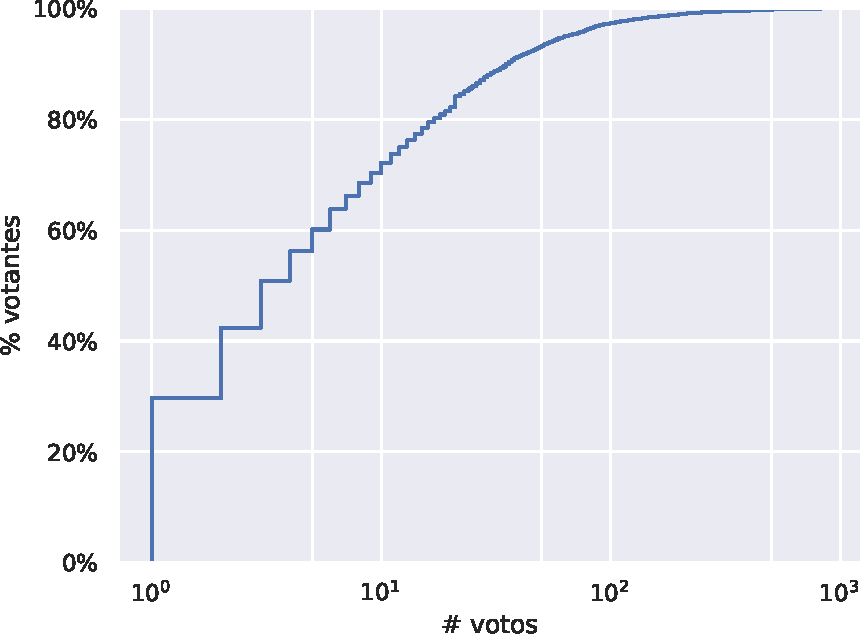
\includegraphics[width=\linewidth]{figures/04_exploracion/04_hybrid_ecdf_voters_Decentraland.pdf}
        \caption[Función de Dist. Cum. de votos por usuario de Decentraland.]{Función de Distribución Cumulativa de votos por usuario de Decentraland.}
        \label{fig:04-ecdf-voters}
    \end{minipage}\hfill\begin{minipage}{.48\linewidth}
        \centering
        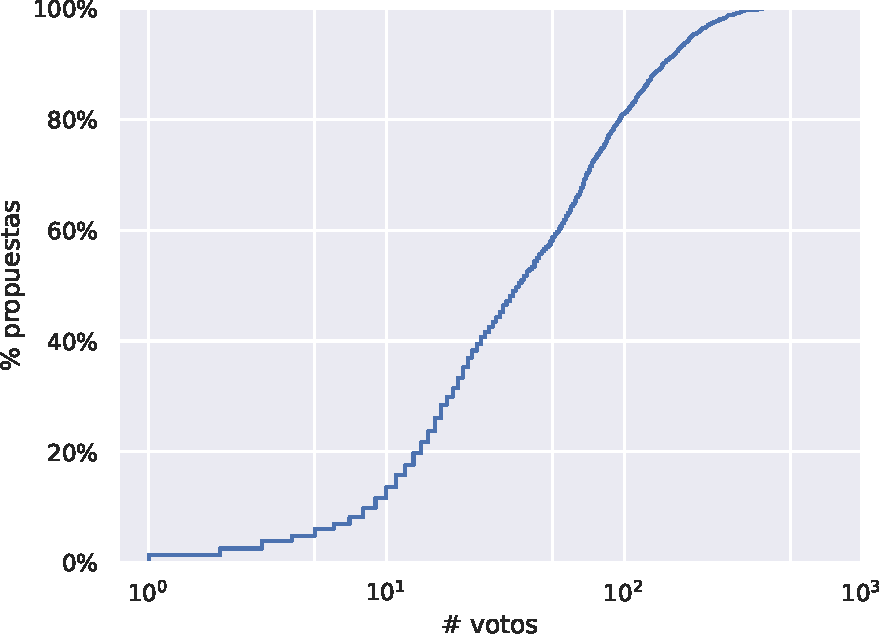
\includegraphics[width=\linewidth]{figures/04_exploracion/04_hybrid_ecdf_proposals_Decentraland.pdf}
        \caption[Función de Dist. Cum. de votos por propuesta de Decentraland.]{Función de Distribución Cumulativa de votos por propuesta de Decentraland.}
        \label{fig:04-ecdg-proposals}
    \end{minipage}
\end{figure}

Su proceso de votación está desplegado en Snapshot, donde se han presentado más de 2~000 propuestas y participan más de 7~000 votantes, emitiendo más de 115~000 votos en total. Sin embargo, como en la mayoría de las \glspl{dao}, la participación es baja, con la mayoría de los miembros votando como mucho en 3 propuestas. Aunque existen 197 miembros (${\sim}2.71\%$) que han emitido más de 100 votos cada uno, la distribución de votos en propuestas de la figura~\ref{fig:04-ecdf-voters} muestra una gran cantidad de usuarios con menos de 10 votos y una pequeña minoría con más de 100.

En cuanto a las propuestas, el grafo es más denso, con una media de 56 votos por propuesta y más de 350 propuestas con más de 100 votos. Sin embargo, la propuesta más votada cuenta con votos de solo el 5\% del total de miembros (385 votos). La figura~\ref{fig:04-ecdg-proposals} muestra de forma detallada la distribución de votos por propuesta en la organización.

% Decentraland ha experimentado un crecimiento gradual en el número de usuarios a lo largo del tiempo, como puede observarse en la figura~\ref{fig:datos-voters-tiempo} lo que plantea el desafío del arranque en frío al tratar con nuevos usuarios. Sin embargo, el problema del cold-start es aún más relevante en relación con las propuestas, pues muchos de esos miembros no volverán a participar. 
Como puede observarse en la figura~\ref{fig:datos-activos-tiempo}, el número de usuarios activos a lo largo del tiempo ha tenido picos de hasta 1~400, pero parece situarse entre los 600 y 800, con una pequeña bajada durante el verano. Además, como se observa en la figura~\ref{fig:rolling_proposals}, se crean entre 10 y 20 propuestas semanalmente, aunque en ocasiones se han observado picos de hasta 70 propuestas, lo que puede dificultar la participación.

La distribución de las propuestas creadas a lo largo de la semana es monotónica y descendente como puede verse en la figura~\ref{fig:04-propuestas-semana}, con casi el doble de propuestas creadas un lunes que en un día de fin de semana.

\begin{figure}[t]
    % \begin{minipage}[t]{.48\linewidth}
    %     \centering
    %     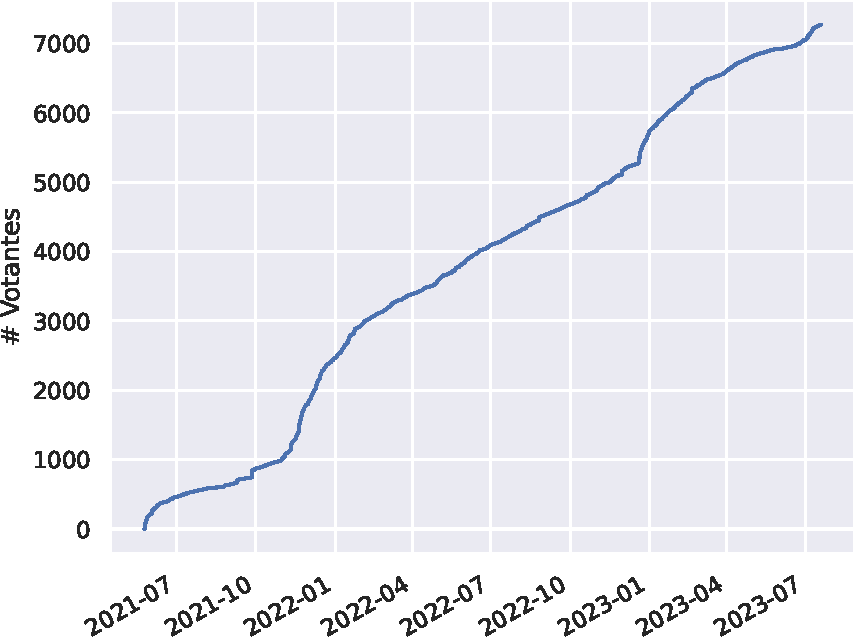
\includegraphics[width=\linewidth]{figures/04_exploracion/04_hybrid_cumcnt_users_Decentraland.pdf}
    %     \caption{Número de usuarios en Decentraland a lo largo del tiempo.}
    %     \label{fig:datos-voters-tiempo}
    % \end{minipage}\hfill%
    \begin{minipage}[t]{.48\linewidth}
        \centering
        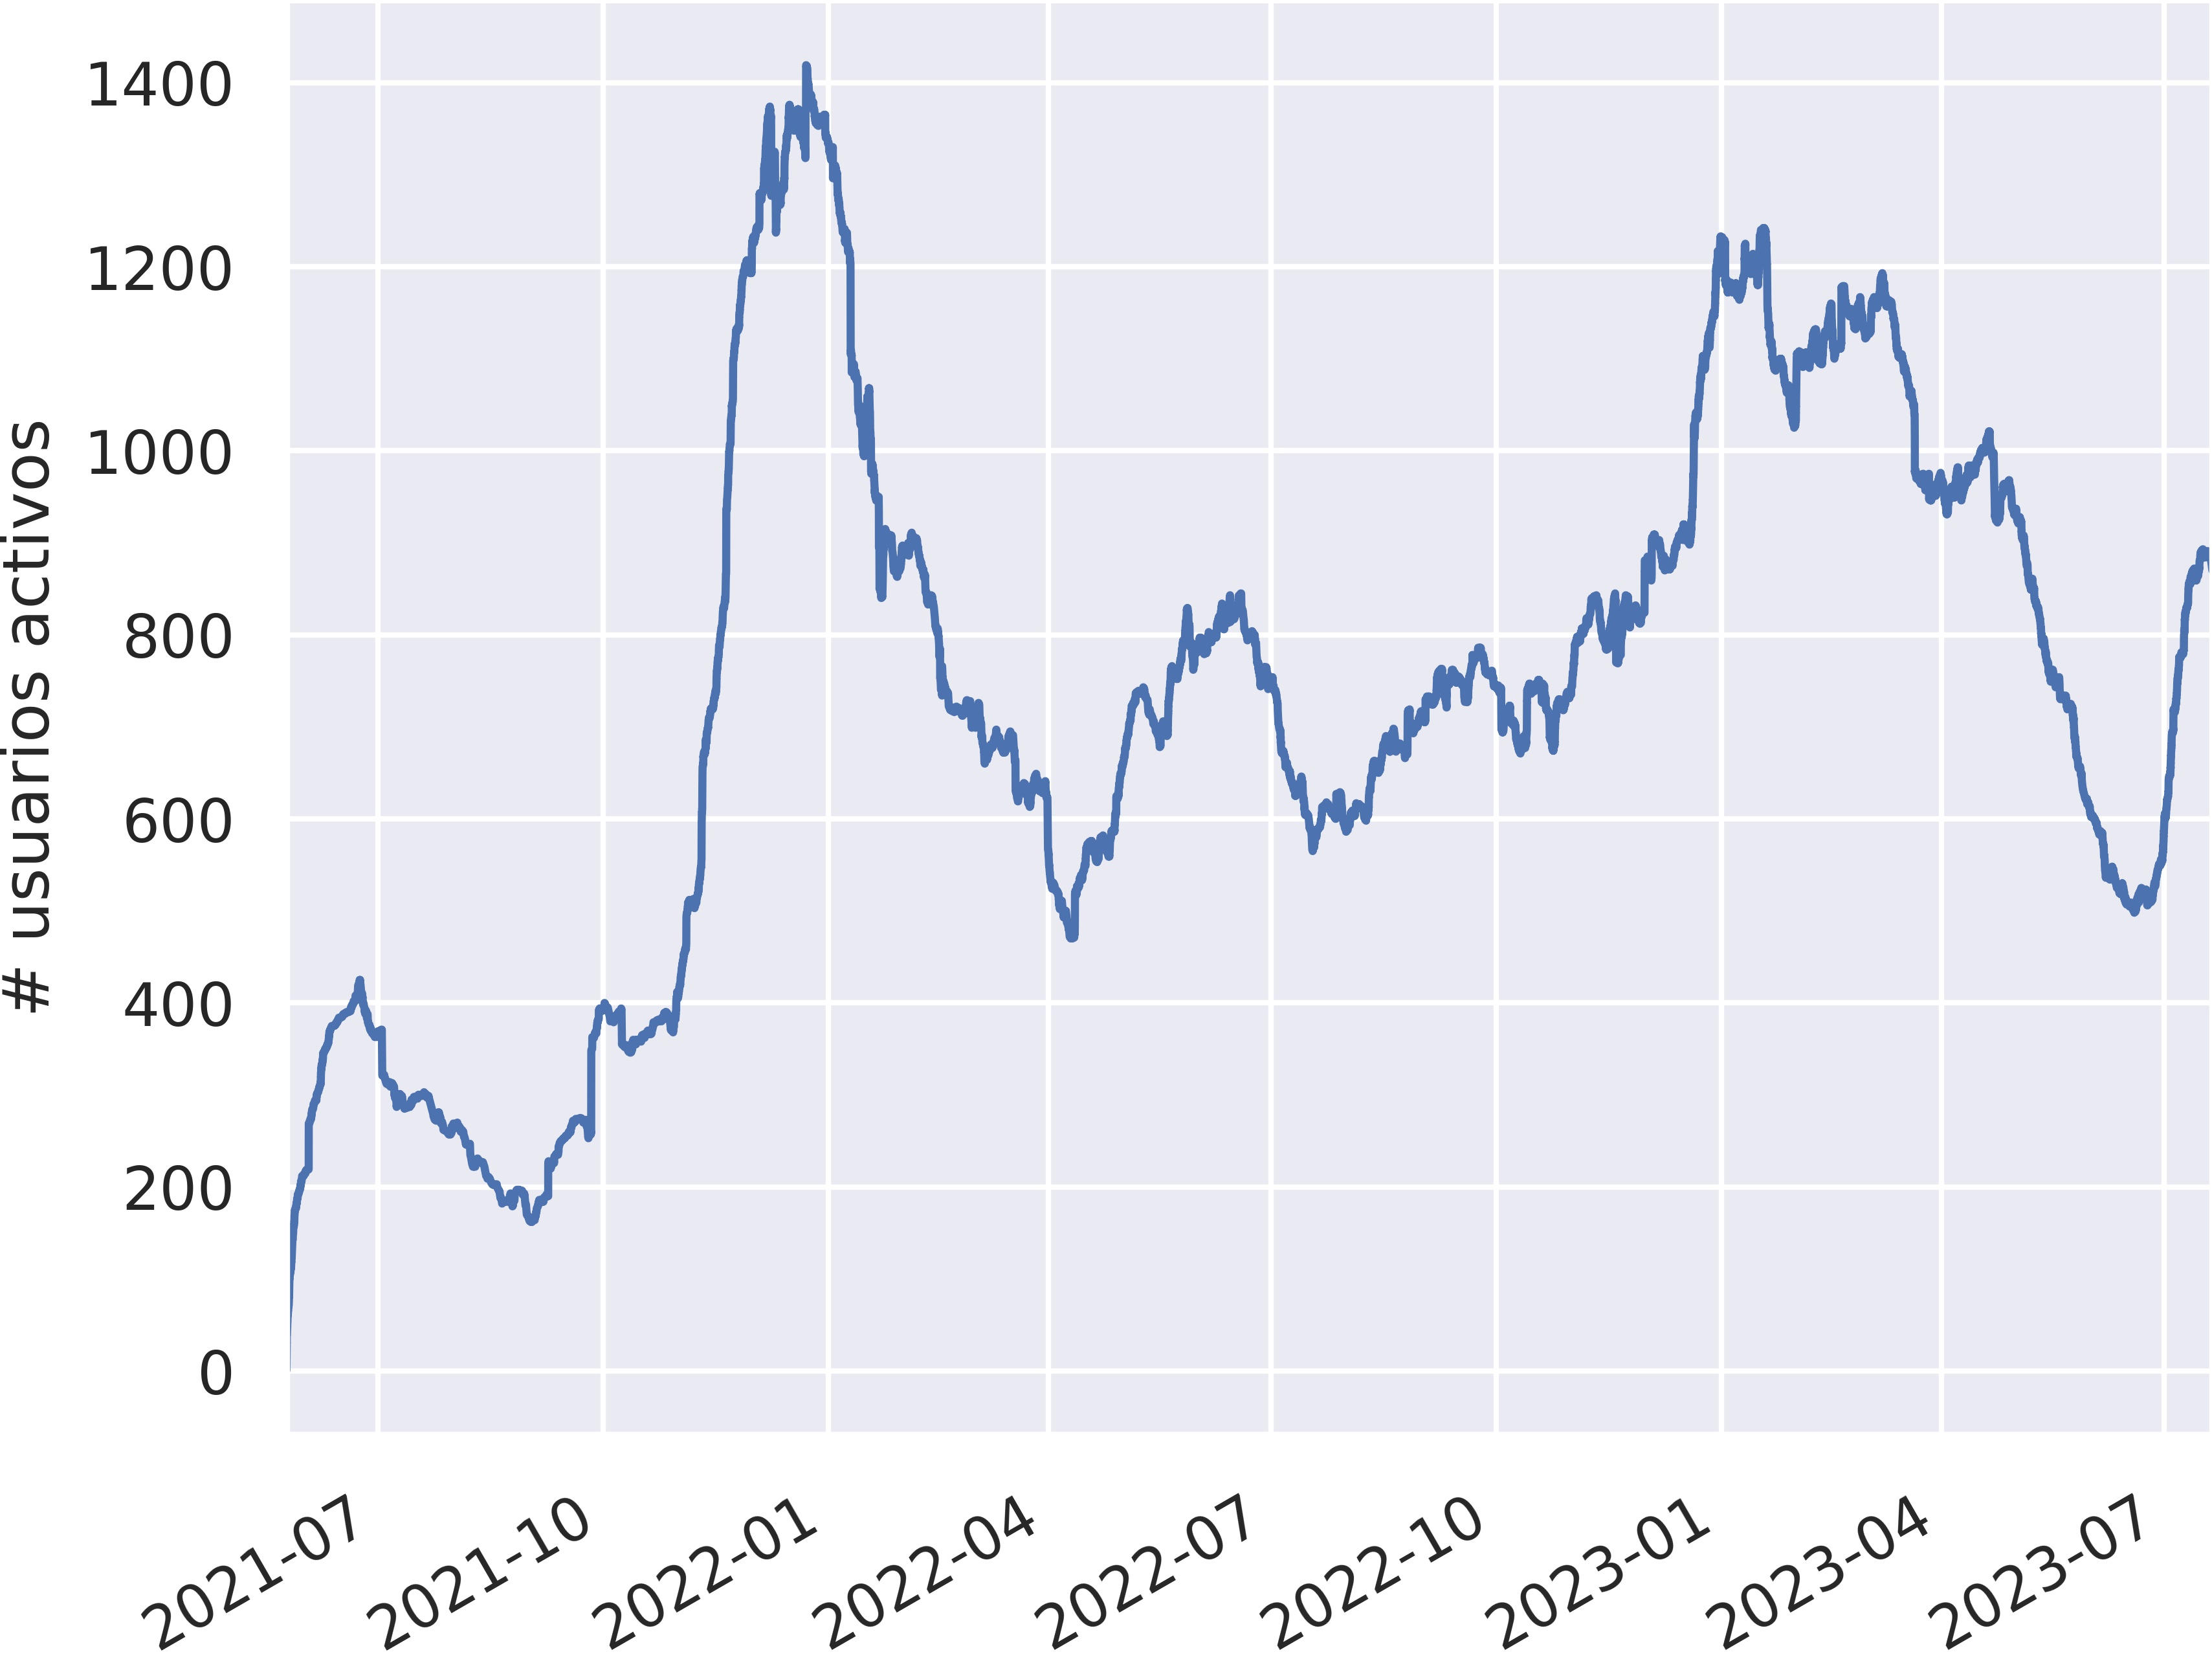
\includegraphics[width=\linewidth]{figures/04_exploracion/04c_rolling_voters_30D_Decentraland.png}
        \caption[Número de usuarios activos en Decentraland a lo largo del tiempo.]{Número de usuarios activos en Decentraland a lo largo del tiempo. Un usuario se considera activo si ha realizado un voto en una propuesta en los últimos 30 días.}
        \label{fig:datos-activos-tiempo}
    \end{minipage}\hfill%
    \begin{minipage}[t]{.48\linewidth}
        \centering
        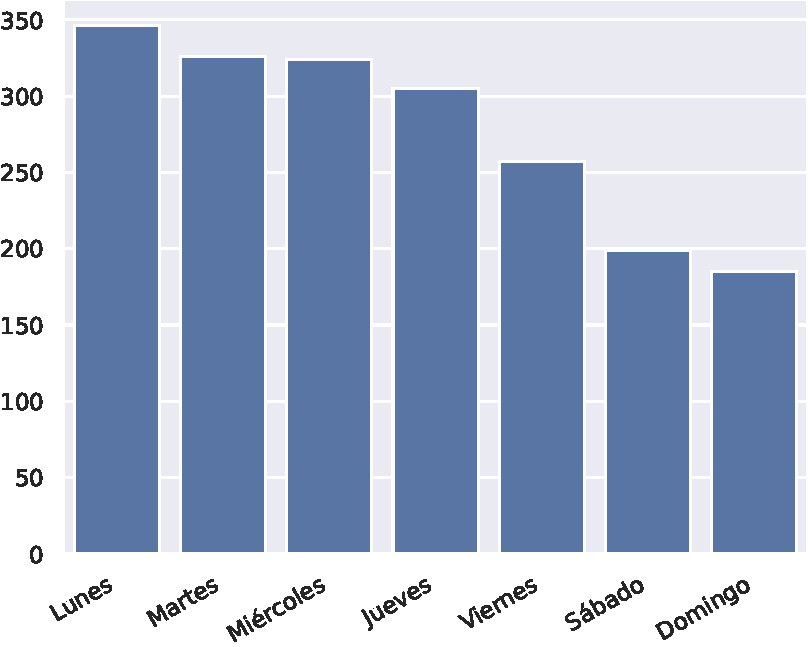
\includegraphics[width=\linewidth]{figures/04_exploracion/04_creation_dow_Decentraland.pdf}
        \caption{Número de propuestas creadas por día de la semana en Decentraland.}
        \label{fig:04-propuestas-semana}
    \end{minipage}
\end{figure}

\begin{figure}[p]
    \centering
    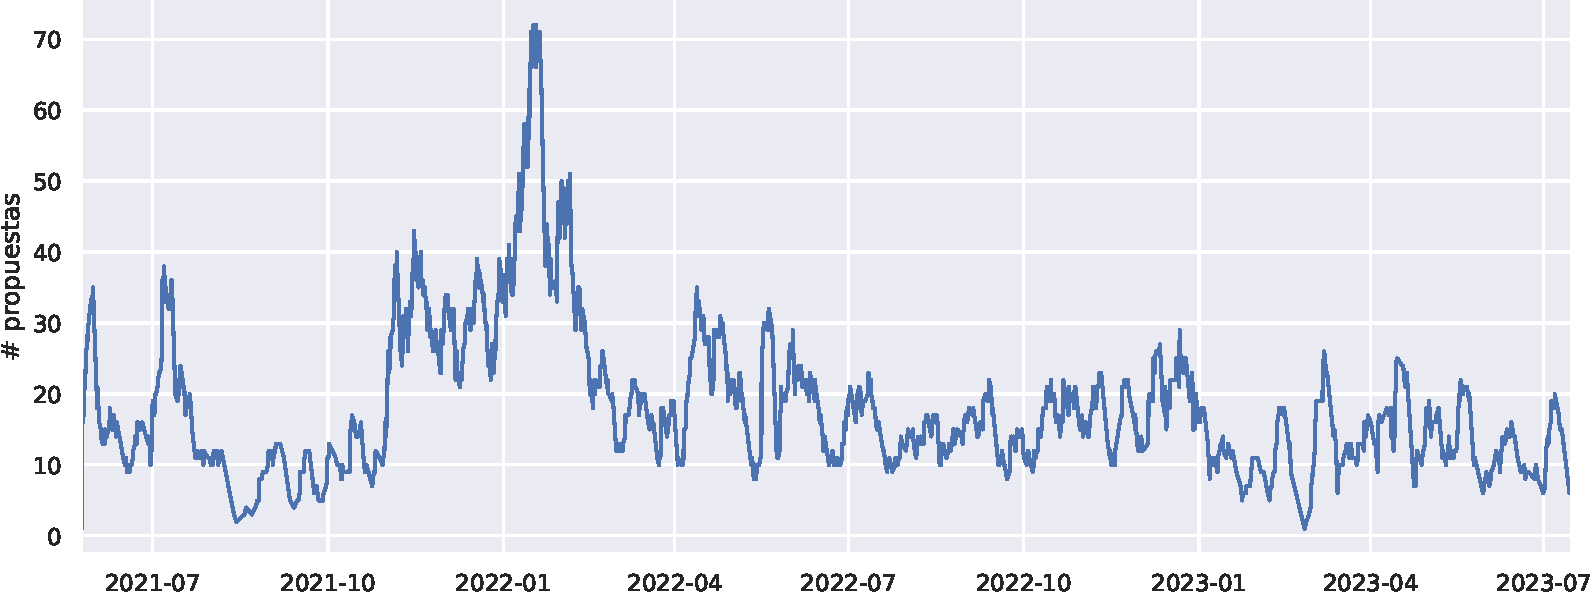
\includegraphics[width=\linewidth]{figures/04_exploracion/04c_rolling_proposals_7D_Decentraland.pdf}
    \caption[Propuestas abiertas en los últimos 7 días en la DAO Decentraland.]{Suma móvil de propuestas abiertas en los últimos 7 días en la \gls{dao} Decentraland.}
    \label{fig:rolling_proposals}
\end{figure}

% \begin{itemize}
    % \item Decentraland es una plataforma de metaverso donde los usuarios pueden comprar parcelas virtuales como \glspl{nft} utilizando criptomonedas basadas en Ethereum. Su desarrollo comenzó en 2015, en 2017 consiguió 26 millones de dólares en su \gls{ico} en la que fue lanzada al público~\cite{higgins_26_2017}, y en 2022 se valoró la plataforma con un valor de 1.2 mil millones de dólares~\cite{tangermann_12_2022}. Ha atraído la atención de grandes marcas como Samsung, Tommy Hilfiger o PricewaterhouseCoopers~\cite{noauthor_decentraland_nodate}, que han comprado \textquote{propiedades} en su mundo, y por lo tanto son miembros con pleno derecho a voto.
    % \item Su mecanismo de organización y votación está desplegado en Snapshot con más de 2~000 propuestas y 7~000 votantes, que han efectuado más de 115~000 votos.
    % \item Sin embargo, como en todas las DAOs, la participación es muy baja. La mayoría de los miembros han efectuado solo 3 votos, pero hay 197 miembros (2.71\%) que han emitido más de 100 votos cada uno, dando una media de 16 votos por votante. En la figura~\ref{fig:04-ecdf-voters} se muestra la distribución cumulativa de votos en propuestas, donde se puede ver que hay una gran mayoría de usuarios con menos de 10 votos, y una pequeña minoría con menos de 100.
    % \item Desde el punto de vista de las propuestas, el grafo es mucho más denso, con una media de 56 votos por propuesta, y hay 367 propuestas con más de 100 votos. Sin embargo, la propuesta con más votos tiene tan solo 385 votos, un 5\% del total de miembros.
    % \item En el caso de Decentraland, se han ido añadiendo usuarios poco a poco a lo largo del tiempo de vida de la organización, por lo que habrá que lidiar con el problema de cold-start con los usuarios, como se ve en la figura~\ref{fig:datos-voters-tiempo}
    % \item Normalmente se generan entre 10 y 20 propuestas a la semana, una cantidad que puede parecer manejable en un principio. Sin embargo, hay épocas en las que se crean 30 propuestas a la semana, y picos de hasta 70, como se puede ver en la figura~\ref{fig:rolling_proposlas}.
    % \item En general los usuarios votan cualquier día de la semana por igual, con menos votos realizados en Domingo. Sin embargo, las propuestas si que forman una distribución de campana con un pico de propuestas creadas en Martes, y muchas menos propuestas creadas de Viernes a Domingo. En general, los usuarios votan en los primeros 2 días de creación de la propuesta, a pesar de que tienen un tiempo de votación de 7 días.
% \end{itemize}

\begin{figure}[p]
    \centering
    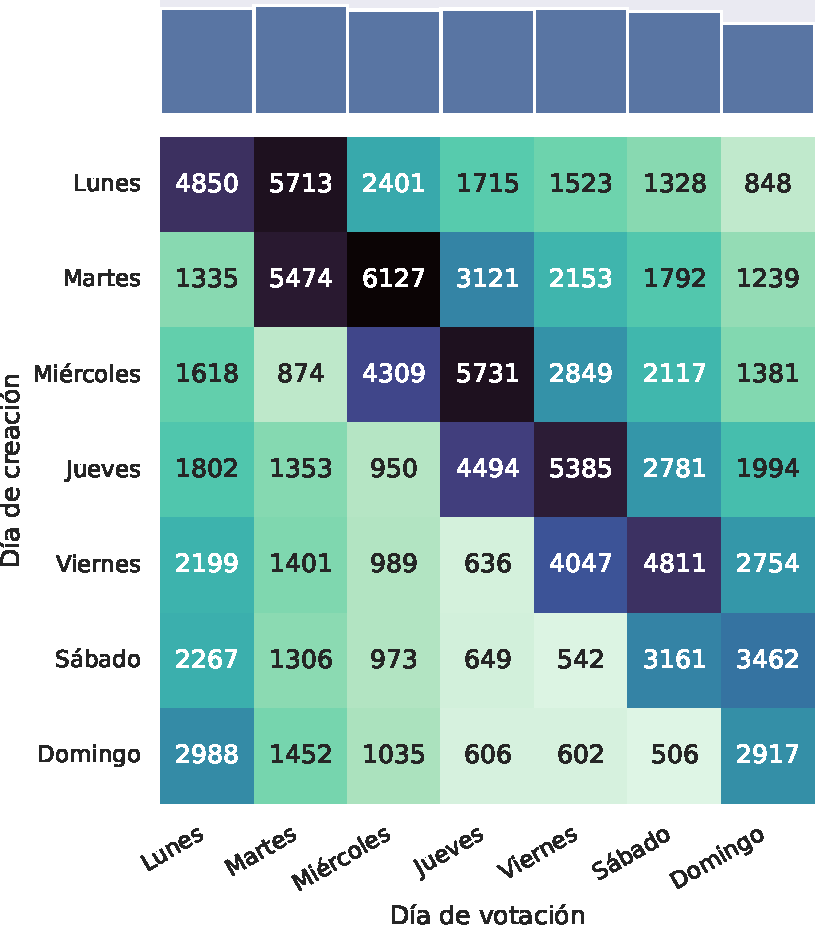
\includegraphics[scale=.8]{figures/04_exploracion/04c_heatmap_proposals_Decentraland.pdf}
    \caption[Mapa de calor día de voto y fecha de creación propuesta.]{Mapa de calor con distribución marginal ilustrando la correlación entre el día en el que se produce un voto y el día de creación de la propuesta en la que se realizó el voto.}
    \label{fig:heatmap-propuestas}
\end{figure}

En las distribuciones marginales de la figura~\ref{fig:heatmap-propuestas}, se pueden observar patrones interesantes en la distribución de los votos y la creación de propuestas en Decentraland a lo largo de los días de la semana. Sobre las votaciones, los usuarios muestran una tendencia uniforme a lo largo de la semana, con una ligera bajada de participación los sábados y domingos, y un ligero repunte los martes, prefiriendo los usuarios la actividad en los días hábiles. % Por otro lado, la distribución de la creación de propuestas es más heterogénea, siguiendo una distribución con una notable campana cuyo máximo es el martes, y una disminución gradual a lo largo de la semana con una marcada reducción de propuestas durante el fin de semana, desde el viernes hasta el domingo.

En la sección central de la figura, se presenta un mapa de calor que ilustra la cantidad de propuestas y votos emitidos cada día de la semana. Se observa que las propuestas reciben la mayor cantidad de votos al día siguiente de su creación, y, a medida que transcurren los días, experimentan una disminución en la cantidad de votos recibidos. Esta regla sólo se rompe los lunes, que puede haber más votos que en Domingo para las propuestas creadas ese día, ya que la participación es menor como se indica en el párrafo anterior.

\section{Propuesta de sistema}

% \begin{itemize}
    % \item Se buscarán modelos probados ya implementados en librerías, uno basado en contenido y otro basado en las relaciones, para realizar las recomendaciones.
    % \item El modelo basado en contenido tendrá sólo en cuenta el título y la descripción de las propuestas, utilizando modelos de \gls{pln}.
    % \item El modelo basado en filtrado colaborativo estará basado en \gls{gnn}, pensando en la expansión del grafo de relaciones más allá de la \gls{dao} en un posible trabajo futuro.
    % \item Se creará un sistema híbrido que combine ambos modelos.
    % \item No se tendrá en cuenta más contexto en ninguno de los dos sistemas. Ninguno de los dos tendrá en cuenta el contexto temporal, pero se les añadirá un pos-filtrado para evitar recomendar propuestas que ya estén cerradas.
    % \item Sin embargo, la evaluación si que tendrá que ser dividiendo los folds en el tiempo, y teniendo en cuenta dicha característica al reportar las métricas.
    % \item Asumiremos que el sistema recomendador se ejecutará periódicamente (por ejemplo, cada semana o cada día), y se evaluará de manera acorde. No se ejecutará de manera continua. Asumimos que el modelo puede ser re-entrenado por completo cada vez que se quieran realizar nuevas recomendaciones.
    % \item Por esa razón, el entrenamiento de los sistemas desarrollados deberían ser rápidos (de varios minutos, como mucho).
% \end{itemize}

En esta sección se realiza una propuesta inicial del posible \gls{sr}. Se buscará utilizar modelos de \glspl{sr} ya validados y disponibles en librerías estándar. Se construirán tres modelos: uno siguiendo un enfoque basado en contenido, otro siguiendo un enfoque basado en \gls{cf}, y un tercero que será un híbrido que combine los otros dos sistemas.

El modelo basado en contenido se limitará a analizar únicamente el título y la descripción de las propuestas, empleando técnicas de \gls{pln}. Por otro lado, el modelo basado en filtrado colaborativo se basará en analizar el grafo bipartito formado por los votantes y las propuestas, utilizando una \gls{gnn}. El sistema híbrido integrará los \textit{rankings} producidos por los dos otros sistemas.

En ninguno de los dos sistemas propuestos se considerará más contexto ni información adicional como el tiempo o día de creación de la propuesta. No obstante, se aplicará un pos-filtrado para evitar recomendar aquellas propuestas cuyo periodo de votación haya concluido. Para ello, el método encargado de realizar las $k$ recomendaciones utilizando el modelo recibirá el conjunto de propuestas consideradas \textit{recomendables}, y se encargará de clasificarlas según su idoneidad, y devolviendo las $k$ mejores recomendaciones para cada usuario.

De esta manera, el modelo se ejecutará en intervalos discretos de tiempo, y la evaluación será en consecuencia. Es decir, asumiendo que el recomendador se ejecutará de forma periódica (por ejemplo, cada semana o cada día) y se evaluará de acuerdo con esta periodicidad. Por ejemplo, para poder enviar un boletín o \textit{newsletter} personalizado con dicha periodicidad y mejorar la participación~\cite{maslowska_effectiveness_2011}. No se contempla la ejecución continua, sino que presupone la posibilidad de reentrenar completamente el modelo en cada ocasión que se desee realizar nuevas recomendaciones. Por consiguiente, uno de los requisitos es que el entrenamiento de los sistemas desarrollados sea rápido, con tiempos de entrenamiento en el orden de minutos.
